\section{Theorie}
\label{sec:Theorie}

Der Franck-Hertz-Versuch gehört zu den Elektronenstoßexperimenten. Dabei werden in einem mit Hg-Dampf gefüllten Glaskolben die Hg-Atome mit Elektronen 
sowohl elastisch wie unelastisch gestoßen. Die Elektronen werden dabei mittels eines Glühdrahtes erzeugt, welcher zusätzlich mit einem Oxid eines 
Erdalkalimetalles bestrichen wird, sodass die Austrittsarbeit niedrig ist und selbst bei geringer Temperatur viele Elektronen emittiert werden.
Um die Energiedifferenz zwischen dem ersten angeregten Zustand und dem Grundzustand zu messen, kann die 
Energiedifferenz der Elektronen vor und nach einem unelastischen Stoß beobachtet werden. Es gilt für die Energiedifferenz der Zustände
\begin{equation*}
    \frac{m_0\cdot v^2_{\symup{vor}}}{2} - \frac{m_0\cdot v^2_{\symup{nach}}}{2} = E_1 - E_0 \; .
\end{equation*}

Gegenüber des Glühdrahtes befindet sich eine netzförmige Elektrode, die die Elektronen mittels einer Gleichspannung $U_{\symup{B}}$ beschleunigt. 
Die kinetische Energie der Elektronen lässt sich über 
\begin{equation*}
    \frac{m_0\cdot v^2_{\symup{vor}}}{2} = e_0U_{\symup{B}}
\end{equation*}
beschreiben.
Hinter der Beschleunigungselektrode befindet sich die Auffängerelektrode, auf der die Elektronen landen und einen Auffängerstrom $I_{\symup{A}}$ erzeugen.
Die Auffängerelektrode besitzt jedoch eine geringe Gegenspannung $U_{\symup{A}}$, durch die Elektronen ein Bremsfeld überwinden müssen. Nur Elektronen, 
die die Ungleichung
\begin{equation*}
    \frac{m_0}{2}v^2_{\symup{z}} \geq e_0U_{\symup{A}}
\end{equation*}
erfüllen, erreichen somit die Auffängerelektrode. 

Im Beschleunigungsraum befinden sich nun Hg-Atome, die mit den Elektronen zusammenstoßen können. Dabei ist zwischen elastischen und unelastischen Stößen 
zu unterscheiden. Wenn die Elektronenenergie gering ist, sind alle Stöße elastisch. Die Energieabgabe des Elektrons and das Hg-Atom ist jedoch aufgrund 
der hohen Massendifferenz vernachlässigbar klein. Die Richtungsänderung des Elektrons kann jedoch erheblich sein. 
Wenn die Elektronendifferenz größer oder gleich der Energiedifferenz $E_1 - E_0$ ist, kann das Elektron das Hg-Atom anregen. Dabei wird die eben 
genannte Energiedifferenz auf das Hg-Atom übertragen und dieses befindet sich im ersten angeregten Zustand. Nach einer kurzen Relaxationszeit, fällt
das Hg-Atom in den Grundzustand zurück und emittiert dabei ein Photon mit eben dieser Energiedifferenz
\begin{equation*}
    \symup{h}\nu = E_1 - E_0 \; .
\end{equation*}

Wenn man $U_{\symup{B}}$ langsam erhöht, wächst der Auffängerstrom $I_{\symup{A}}$ an sobald $U_{\symup{B}}$ die Gegenspannung $U_{\symup{A}}$ 
übersteigt. Der Auffängerstrom erreicht sein Maximum bei einer Elektronenenergie $E_1 - E_0$, da nun auch unelastische Stöße stattfinden, bei denen
die Elektronen diese Energie an die Hg-Atome abgeben. Nun können die Elektronen das Bremsfeld nicht mehr überwinden. In Folge dessen fällt der 
Auffängerstrom ab. Wenn $U_{\symup{B}}$ weiter ansteigt, können die Elektronen erneut Energie aufnehmen, sodass der Auffängerstrom wieder ansteigt 
bis ein zweiter unelastischer Stoß stattfinden kann. Der Verlauf des Auffängerstroms ist in \autoref{fig:fhkurve} dargestellt. 
\begin{figure}
    \centering
    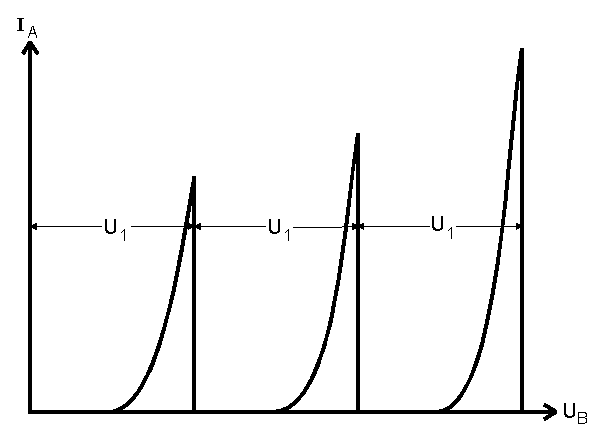
\includegraphics[height = 9cm]{fhkurve.pdf}
    \caption{Abhängigkeit des Auffängerstroms $I_{\symup{A}}$ von der Beschleunigerspannung $U_{\symup{B}}$ \cite{ap601}.}
    \label{fig:fhkurve}
\end{figure}

Der Abstand $U_1$ zwischen aufeinanderfolgenden Maxima stimmt dabei mit dem ersten Anregungspotential überein
\begin{equation*}
    U_1 = \frac{1}{e_0}\left(E_1 - E_0\right) \; .
\end{equation*}

\subsection{Nebeneffekte mit Einfluss auf die Franck-Hertz-Kurve}
Das Beschleunigungspotential $U_{\symup{B}}$ wird um das Kontaktpotential 
\begin{equation*}
    K = \frac{1}{e_0} \left(\Phi_{\symup{B}}-\Phi_{\symup{G}}\right)
\end{equation*}
reduziert, wenn die Elektroden aus Materialien mit unterschiedlicher Austrittsarbeit bestehen. Um eine hohe Emissionsrate bei niedriger Temperatur zu 
erzielen, wählt man für den Glühdraht ein Material, dessen Austrittarbeit $\Phi_{\symup{G}}$ viel kleiner als die der Beschleunigungselektrode 
$\Phi_{\symup{B}}$ ist.
Außerdem ist die Franck-Hertz-Kurve um den Wert K verschoben.

Desweiteren besitzen die emittierten Elektronen bereits ein Energiespektrum nach der Fermi-Dirac-Verteilung. Dies führt dazu, dass die Elektronen 
mit unterschiedlichen Anfangsgeschwindigkeiten emittiert werden. Daraus entsteht eine Energieverteilung, die bei $U_{\symup{B_eff}}$ beginnt.
Insgesamt wird der Anstieg beim Annähern an das Maximum verringert und die Franck-Hertz-Kurve fällt nicht mehr auf den Wert 0 ab, sondern nu bis 
zu einem Minimum. 
Außerdem führen die elastischen Stöße mit den Hg-Atomen zu Richtungsänderungen der Elektronen, sodass nicht mehr alle Elektronen die Auffängerelektrode 
erreichen. Dies führt insgesamt zu einer Verbreiterung und einer Abflachung der Franck-Hertz-Kurve.

Damit überhaupt Zusammenstöße zwischen Elektronen und Hg-Atomen zustande kommen, muss die mittlere freie Weglänge der Atome
\begin{equation*}
    \bar{w} [cm] = \frac{0.0029}{p_{\symup{sät}}} [mbar]
\end{equation*}
klein gegenüber dem Abstand a zwischen Glühkathode und Beschleunigungselektrode sein. Dabei ist $p_{\symup{sät}}$ der Sättigungsdampfdruck, der 
aus der Dampfdruckkurve mit
\begin{equation*}
    p_{\symup{sät}}(T) = 5.5 \cdot 10^7 exp\left(\frac{6876}{T}\right)
\end{equation*}
berechnet werden kann. Damit kann eine Temperatur bestimmt werden, bei der der Franck-Hertz-Effekt zu beobachten ist. 

Wenn der Dampfdruckbereich unterschritten wird, durchlaufen die Elektronen ohne Wechselwirkung den Glaskolben. Bei einem zu großen Druck gibt es 
viele elastische Stöße, die zu Richtungsänderungen der Elektronen führen.  
